\documentclass[twoside]{mfitjournal}
\usepackage{amsbib}
\usepackage[T2A]{fontenc}
\usepackage[utf8]{inputenc}
\usepackage[russian]{babel}
\usepackage{amsmath}
\usepackage{graphicx}
\usepackage{geometry}
\usepackage{array}
\usepackage{booktabs}
\usepackage{caption}
\usepackage{float}
\clubpenalty=10000
\widowpenalty=10000
\newcommand{\MFITnumber}{}
\newcommand{\MFITom}{}
\newcommand{\MFITyear}{}
\newcommand{\ISSN}{}
\newcommand{\OISSN}{}
\newcommand{\DOI}{}
\renewcommand{\firstpage}{}
\renewcommand{\lastpage}{}
\SECC{}
\ESECC{}
\geometry{margin=2cm}
\setlength{\headheight}{15pt}
\captionsetup{font=small, labelfont=bf}

\begin{document}

\rustitle{Лабораторная работа 4.2.1. Кольца Ньютона}
\shorttitle{Лабораторная работа 4.2.1}
\author{Евгений Иванов}
\shortauthor{Иванов Е.\,И.}
\institute{МФТИ, группа 5-407}
\email{E-mail:}{}
\rcopyr{Евгений Иванов}

\makeatletter
\renewcommand{\tit}{}
\renewcommand{\@oddhead}{}
\renewcommand{\@evenhead}{}
\makeatother

\pagestyle{fancy}
\fancyhf{}
\fancyhead[RE]{Иванов Е.\,И.}
\fancyhead[LO]{Лабораторная работа 4.2.1}
\cfoot{\arabic{page}}

\maketitle

\section*{Цель работы}

Изучить интерференцию в тонких плёнках на примере колец Ньютона, определить радиус кривизны линзы по зависимости квадратов радиусов колец от их номера и по фотографии картины биений оценить разность длин волн жёлтой и зелёной линий ртути.

\section*{Оборудование и установка}

В работе использовались измерительный микроскоп с опак-иллюминатором, плосковыпуклая линза, пластинка из чёрного стекла, ртутная лампа, щель, линзы, призма прямого зрения и объектная шкала. Наблюдение велось в отражённом свете.

\section*{Краткая теория}

Кольца Ньютона возникают при интерференции волн, отражённых от границ тонкой воздушной прослойки между плосковыпуклой линзой и стеклянной пластинкой. При отражении от оптически более плотной среды возникает фазовый скачок $\pi$, поэтому в центре системы в отражённом свете наблюдается тёмное пятно.

Для малой толщины зазора $d \ll R$ и радиуса кольца $r$ выполняются соотношения
\begin{equation}
r^2 \approx 2Rd,
\end{equation}
\begin{equation}
\Delta = 2d + \frac{\lambda}{2} = \frac{r^2}{R} + \frac{\lambda}{2}.
\end{equation}
Для тёмных колец получается
\begin{equation}
r_m^2 = m \lambda R,
\end{equation}
где $m$ --- номер кольца, $\lambda$ --- длина волны, $R$ --- радиус кривизны линзы. Следовательно, график $r_m^2(m)$ должен быть линейным, а его наклон равен $\lambda R$.

Для двух близких длин волн участки максимальной чёткости интерференционной картины повторяются через $\Delta m$ колец. Из условия наложения двух картин следует оценка
\begin{equation}
\Delta \lambda \approx \frac{\lambda}{\Delta m}.
\end{equation}

\section*{Исходные данные}

Координата центра системы колец восстанавливалась из файла измерений по более точному отсчёту
\[
x_c = 0.415\ \text{см}.
\]
При обработке использовалась цена деления $0.1$ мм на одно деление шкалы, поэтому исходные отсчёты были пересчитаны в сантиметры.
Для каждого кольца координата вычислялась по правилу
\begin{equation}
x_n = \lfloor l \rfloor + \frac{d}{100},
\end{equation}
после чего радиус находился как
\begin{equation}
r_n = |x_n - x_c|.
\end{equation}

\begin{table}[H]
\centering
\caption{Точки для графика $r_n^2(n)$}
\begin{tabular}{ccccccc}
\toprule
$n$ & $l$ & $d$ & $x_n$, см & $r_n$, см & $r_n^2$, $10^{-4}$ см$^2$ & Статус \\
\midrule
1  & 5.25 & 20.0 & 0.052 & 0.010 & 1.1 & в аппроксимации \\
2  & 5.50 & 49.0 & 0.055 & 0.013 & 1.8 & в аппроксимации \\
3  & 5.75 & 77.0 & 0.058 & 0.016 & 2.6 & в аппроксимации \\
4  & 6.00 & 98.0 & 0.070 & 0.028 & 8.0 & исключена \\
5  & 6.25 & 23.0 & 0.062 & 0.021 & 4.3 & в аппроксимации \\
6  & 6.40 & 41.0 & 0.064 & 0.023 & 5.1 & в аппроксимации \\
7  & 6.50 & 57.0 & 0.066 & 0.024 & 5.9 & в аппроксимации \\
8  & 6.75 & 75.0 & 0.068 & 0.026 & 6.8 & в аппроксимации \\
9  & 7.80 & 9.0  & 0.071 & 0.029 & 8.6 & в аппроксимации \\
10 & 8.00 & 0.5  & 0.080 & 0.039 & 15 & исключена \\
\bottomrule
\end{tabular}
\end{table}

В таблице видно, что точка $n=4$ нарушает монотонность радиусов, а точка $n=10$ заметно выбивается как крайняя. Поэтому для итоговой линейной аппроксимации использовались только точки $n = 1,2,3,5,6,7,8,9$.

\section*{Обработка результатов}

Линейная аппроксимация дала
\begin{equation}
r^2 = \bigl[(0.88 \pm 0.05)\,n + (-0.01 \pm 0.27)\bigr]\cdot 10^{-4}\ \text{см}^2,
\end{equation}
при этом коэффициент детерминации составил
\[
R^2 = 0.98.
\]
Для зелёной линии ртути $\lambda = 546.1$ нм радиус кривизны равен
\begin{equation}
R = \frac{a}{\lambda} = (1.6 \pm 0.1)\ \text{см},
\end{equation}
где $a$ --- коэффициент наклона графика $r^2(n)$.

Диаметр центрального пятна соприкосновения, записанный при измерениях как $D \approx 5.6$ деления шкалы, соответствует примерно $0.056$ см. Эта величина задаёт размер центральной области контакта, где сильнее всего проявляются деформации и где теория тонкой воздушной прослойки работает хуже.

\begin{figure}[H]
\centering
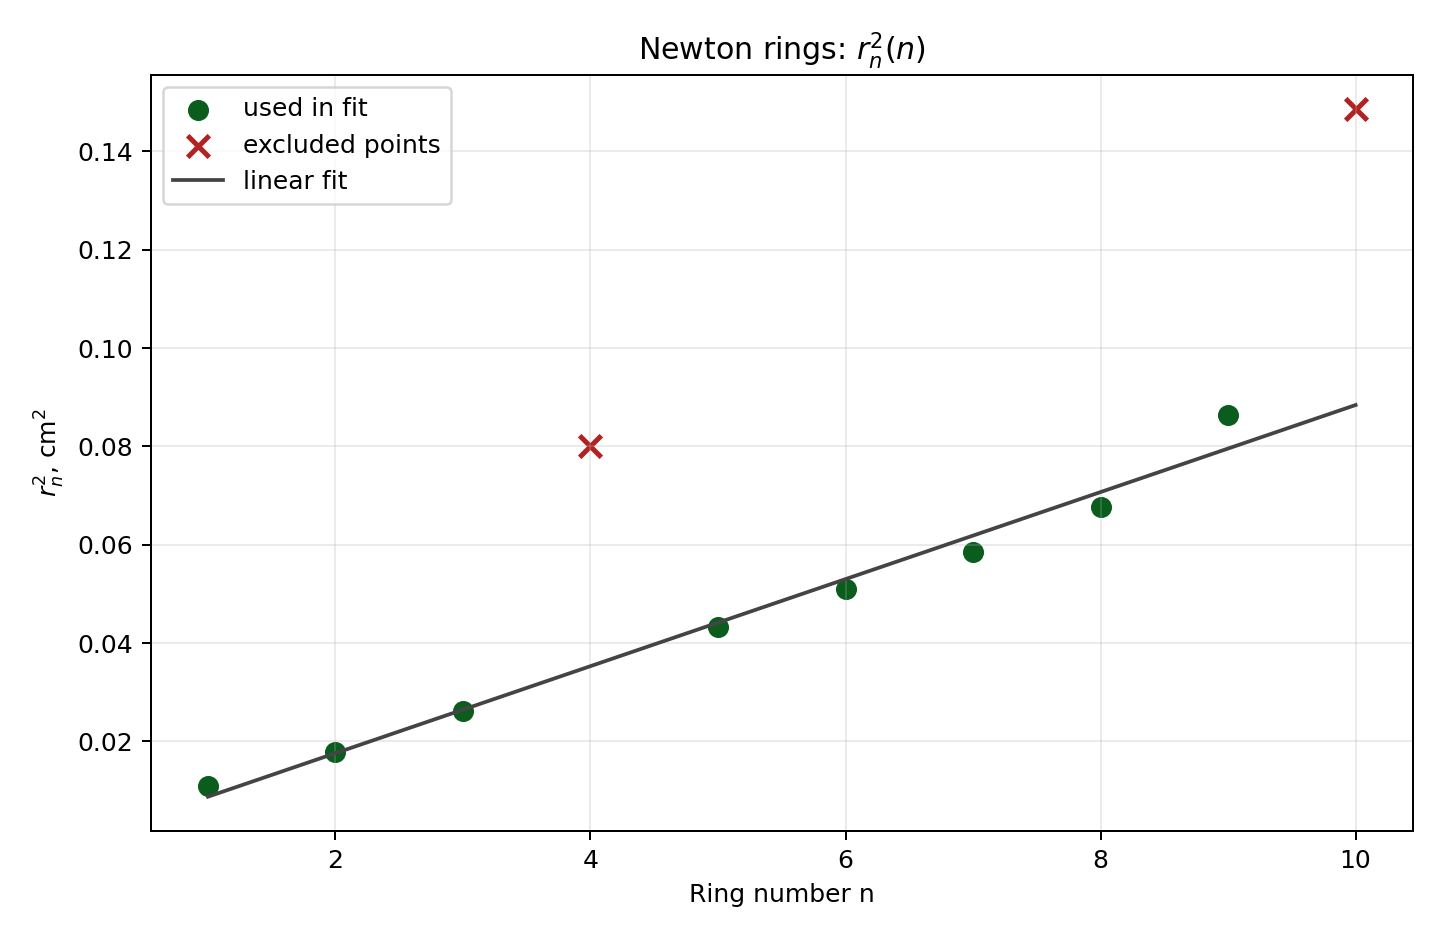
\includegraphics[width=0.83\textwidth]{ring_fit.png}
\caption{График $r_n^2(n)$. Серым показана линейная аппроксимация по точкам $n=1,2,3,5,6,7,8,9$; точки $n=4$ и $n=10$ исключены из подгонки.}
\end{figure}

\section*{Биения по фотографии}

Для снимка ``фото биений.jpg'' сначала определялось положение пятна, вокруг которого идут концентрические кольца. После этого код проводил много пробных прямых через найденный центр под разными углами и выбирал ту, для которой профиль лучше всего показывает последовательность ``чёткие кольца $\to$ зона биений $\to$ снова чёткие кольца''. В итоговой обработке использовался луч, проходящий через центр пятна $(2293,\ 1865)$ px под углом $-10^\circ$ к горизонтали.

\begin{table}[H]
\centering
\caption{Точки, использованные для оценки периода биений}
\begin{tabular}{p{3.3cm}p{9.0cm}}
\toprule
Величина & Значение \\
\midrule
Центр пятна & $(2293,\ 1865)$ px \\
Направление луча & $-10^\circ$ к горизонтали \\
Рабочая ветвь профиля & от центра влево-вверх \\
Число тёмных колец между максимумами огибающей & $\Delta m = 17$ \\
\bottomrule
\end{tabular}
\end{table}

Полный массив точек профиля интенсивности был рассчитан кодом и сохранён в файле ``beat\_profile.csv''. Для оценки периода биений использовались два соседних максимума видности на выбранной ветви и число тёмных колец между ними. Тогда
\begin{equation}
\Delta \lambda \approx \frac{\lambda_{\text{green}}}{\Delta m}
= \frac{546\ \text{нм}}{17}
= 32\ \text{нм}.
\end{equation}
Табличная разность длин волн для линий $579.1$ нм и $546.1$ нм равна
\[
\Delta \lambda_{\text{tab}} = 33\ \text{нм}.
\]

\begin{table}[H]
\centering
\caption{Точки, отображённые на графике интенсивности}
\scriptsize
\begin{tabular}{cccccccc}
\toprule
$s$, px & $I$ & $s$, px & $I$ & $s$, px & $I$ & $s$, px & $I$ \\
\midrule
-0 & 217.1 & 10 & 217.2 & 20 & 216.5 & 30 & 213.8 \\
40 & 212.1 & 50 & 211.4 & 60 & 209.9 & 70 & 209.0 \\
80 & 209.0 & 90 & 208.1 & 100 & 207.9 & 110 & 208.2 \\
120 & 208.2 & 130 & 207.0 & 140 & 207.0 & 150 & 206.3 \\
160 & 206.0 & 170 & 204.6 & 180 & 204.1 & 190 & 205.2 \\
200 & 207.7 & 210 & 209.9 & 220 & 208.7 & 230 & 207.6 \\
240 & 206.5 & 250 & 205.7 & 260 & 205.4 & 270 & 206.9 \\
280 & 212.9 & 290 & 216.8 & 300 & 216.6 & 310 & 218.1 \\
320 & 215.7 & 330 & 216.0 & 340 & 216.9 & 350 & 220.4 \\
360 & 228.3 & 370 & 225.2 & 380 & 218.6 & 390 & 212.4 \\
400 & 208.9 & 410 & 206.8 & 420 & 199.2 & 430 & 196.2 \\
440 & 195.6 & 450 & 195.9 & 460 & 201.6 & 470 & 207.1 \\
480 & 219.3 & 490 & 224.2 & 500 & 221.2 & 510 & 223.1 \\
520 & 227.5 & 530 & 228.3 & 540 & 225.7 & 550 & 214.1 \\
560 & 202.6 & 570 & 197.9 & 580 & 198.7 & 590 & 202.6 \\
600 & 211.1 & 610 & 220.6 & 620 & 229.0 & 630 & 228.6 \\
640 & 222.7 & 650 & 214.5 & 660 & 205.8 & 670 & 200.7 \\
680 & 200.8 & 690 & 206.1 & 700 & 211.7 & 710 & 215.4 \\
720 & 218.9 & 730 & 223.2 & 740 & 219.5 & 750 & 211.3 \\
760 & 208.9 & 770 & 206.5 & 780 & 210.8 & 790 & 215.8 \\
800 & 221.9 & 810 & 214.7 & 820 & 204.4 & 830 & 207.3 \\
840 & 208.7 & 850 & 202.0 & 860 & 197.4 & 870 & 208.2 \\
880 & 209.9 & 890 & 209.6 & 900 & 210.6 & 910 & 211.9 \\
920 & 213.6 & 930 & 214.1 & 940 & 212.1 & 950 & 207.2 \\
960 & 206.3 & 970 & 205.1 & 980 & 201.9 & 990 & 193.3 \\
1000 & 199.2 & 1010 & 205.3 & 1020 & 204.9 & 1030 & 203.2 \\
1040 & 202.2 & 1050 & 205.9 & 1060 & 212.0 & 1070 & 213.3 \\
1080 & 213.0 & 1090 & 209.0 & 1100 & 204.1 & 1110 & 203.4 \\
1120 & 204.1 & 1130 & 204.5 & 1140 & 206.0 & 1150 & 206.6 \\
1160 & 207.8 & 1170 & 213.0 & 1180 & 219.1 & 1190 & 221.5 \\
1200 & 216.9 & 1210 & 212.7 & 1220 & 212.1 & 1230 & 211.3 \\
1240 & 212.0 & 1250 & 219.2 & 1260 & 220.2 & 1270 & 219.7 \\
1280 & 216.9 & 1290 & 211.2 & 1300 & 206.5 & 1310 & 208.9 \\
1320 & 212.5 & 1330 & 213.7 & 1340 & 204.3 & 1350 & 204.0 \\
1360 & 210.0 & 1370 & 214.2 & 1380 & 208.5 & 1390 & 202.6 \\
1400 & 209.1 & 1410 & 213.1 & 1420 & 211.0 & 1430 & 208.1 \\
1440 & 210.7 & 1450 & 212.1 & 1460 & 207.7 & 1470 & 208.0 \\
1480 & 210.1 & 1490 & 210.6 & 1500 & 207.1 & 1510 & 210.8 \\
1520 & 213.5 & 1530 & 211.9 & 1540 & 209.4 & 1550 & 211.5 \\
1560 & 214.3 & 1570 & 211.3 & 1580 & 209.2 & 1590 & 210.0 \\
1600 & 208.4 & 1610 & 206.5 & 1620 & 209.8 & 1630 & 210.2 \\
1640 & 209.7 & 1650 & 207.6 & 1660 & 207.0 & 1670 & 207.1 \\
1680 & 207.2 & 1690 & 206.2 & 1700 & 205.7 & 1710 & 205.7 \\
1720 & 206.5 & 1730 & 207.0 & 1740 & 206.1 & 1750 & 204.6 \\
1760 & 202.2 & 1770 & 198.7 & 1780 & 195.5 & 1790 & 192.7 \\
1800 & 189.0 & 1810 & 185.5 & 1820 & 183.0 & 1830 & 178.8 \\
1840 & 174.0 & 1850 & 167.6 & 1860 & 159.6 & 1870 & 153.8 \\
1880 & 142.3 & 1890 & 136.7 & 1900 & 132.6 & 1910 & 122.2 \\
1920 & 116.1 & 1930 & 111.0 & 1940 & 107.3 & 1950 & 104.5 \\
1960 & 98.4 & 1970 & 96.8 & 1980 & 89.5 & 1990 & 86.0 \\
2000 & 77.6 & 2010 & 74.6 & 2020 & 71.2 & 2030 & 68.8 \\
2040 & 66.0 & 2050 & 65.1 & 2060 & 61.6 & 2070 & 55.8 \\
2080 & 52.3 & 2090 & 48.9 & 2100 & 44.2 & 2110 & 41.6 \\
2120 & 41.6 & 2130 & 39.2 & 2140 & 34.7 & 2150 & 31.7 \\
2160 & 33.0 &  &  &  &  &  &  \\
\bottomrule
\end{tabular}
\end{table}

\begin{figure}[H]
\centering
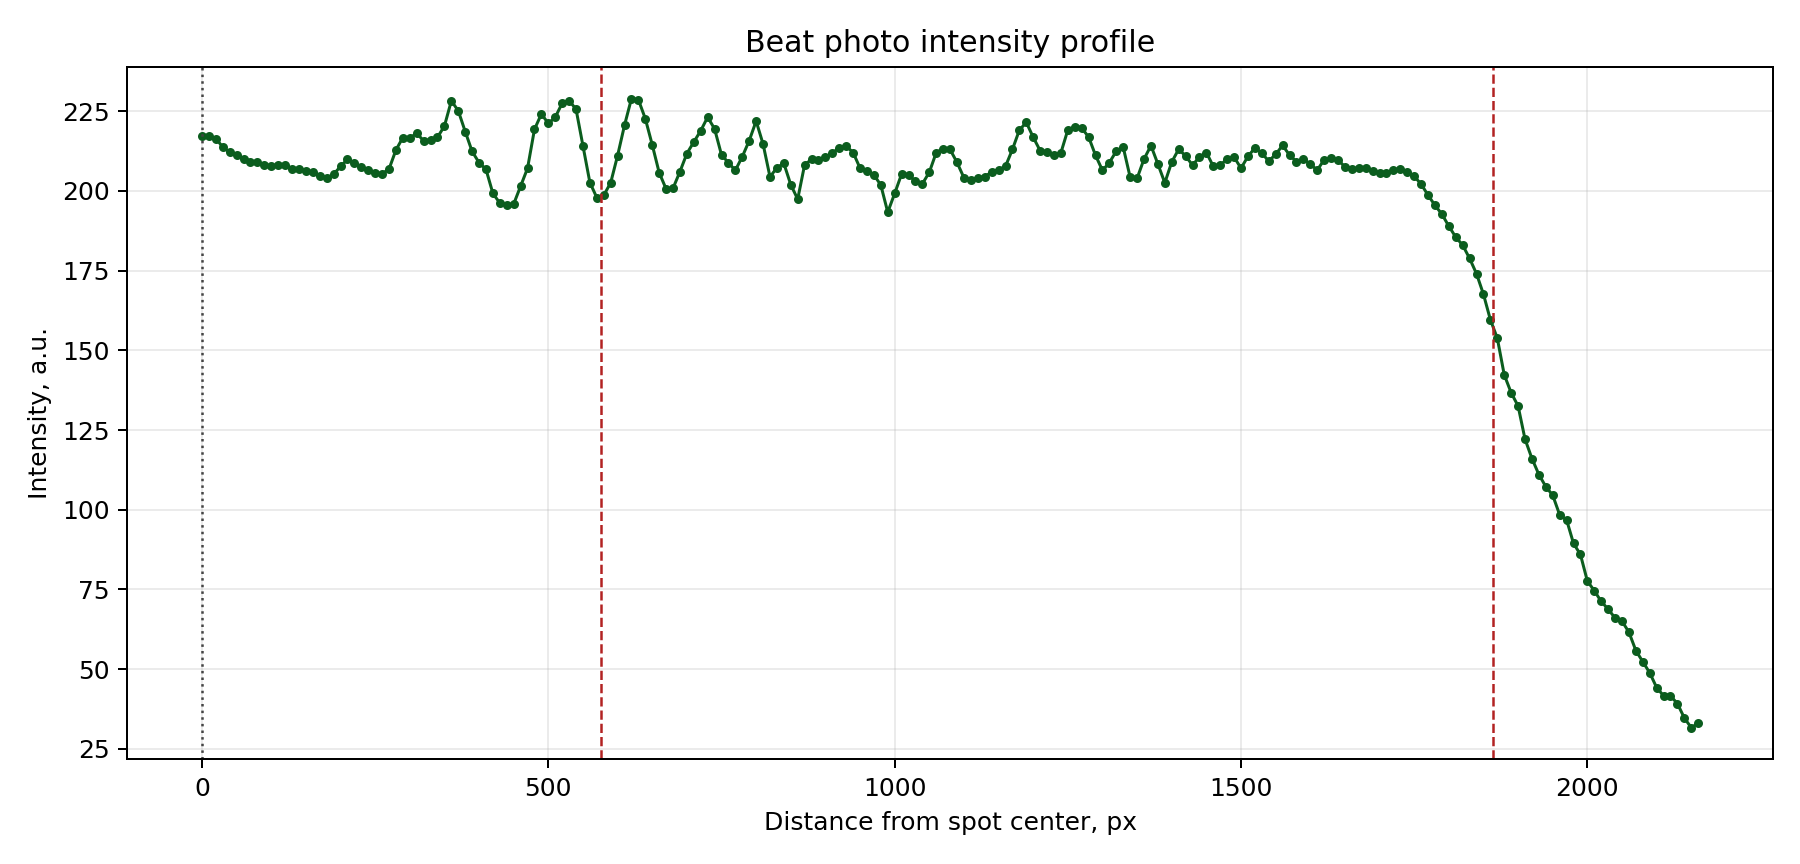
\includegraphics[width=0.90\textwidth]{beat_profile.png}
\caption{Профиль интенсивности вдоль выбранного луча через центр пятна. По оси абсцисс отложено расстояние от центра; пунктиром отмечены два соседних максимума видности, между которыми проводился счёт колец.}
\end{figure}

\begin{figure}[H]
\centering
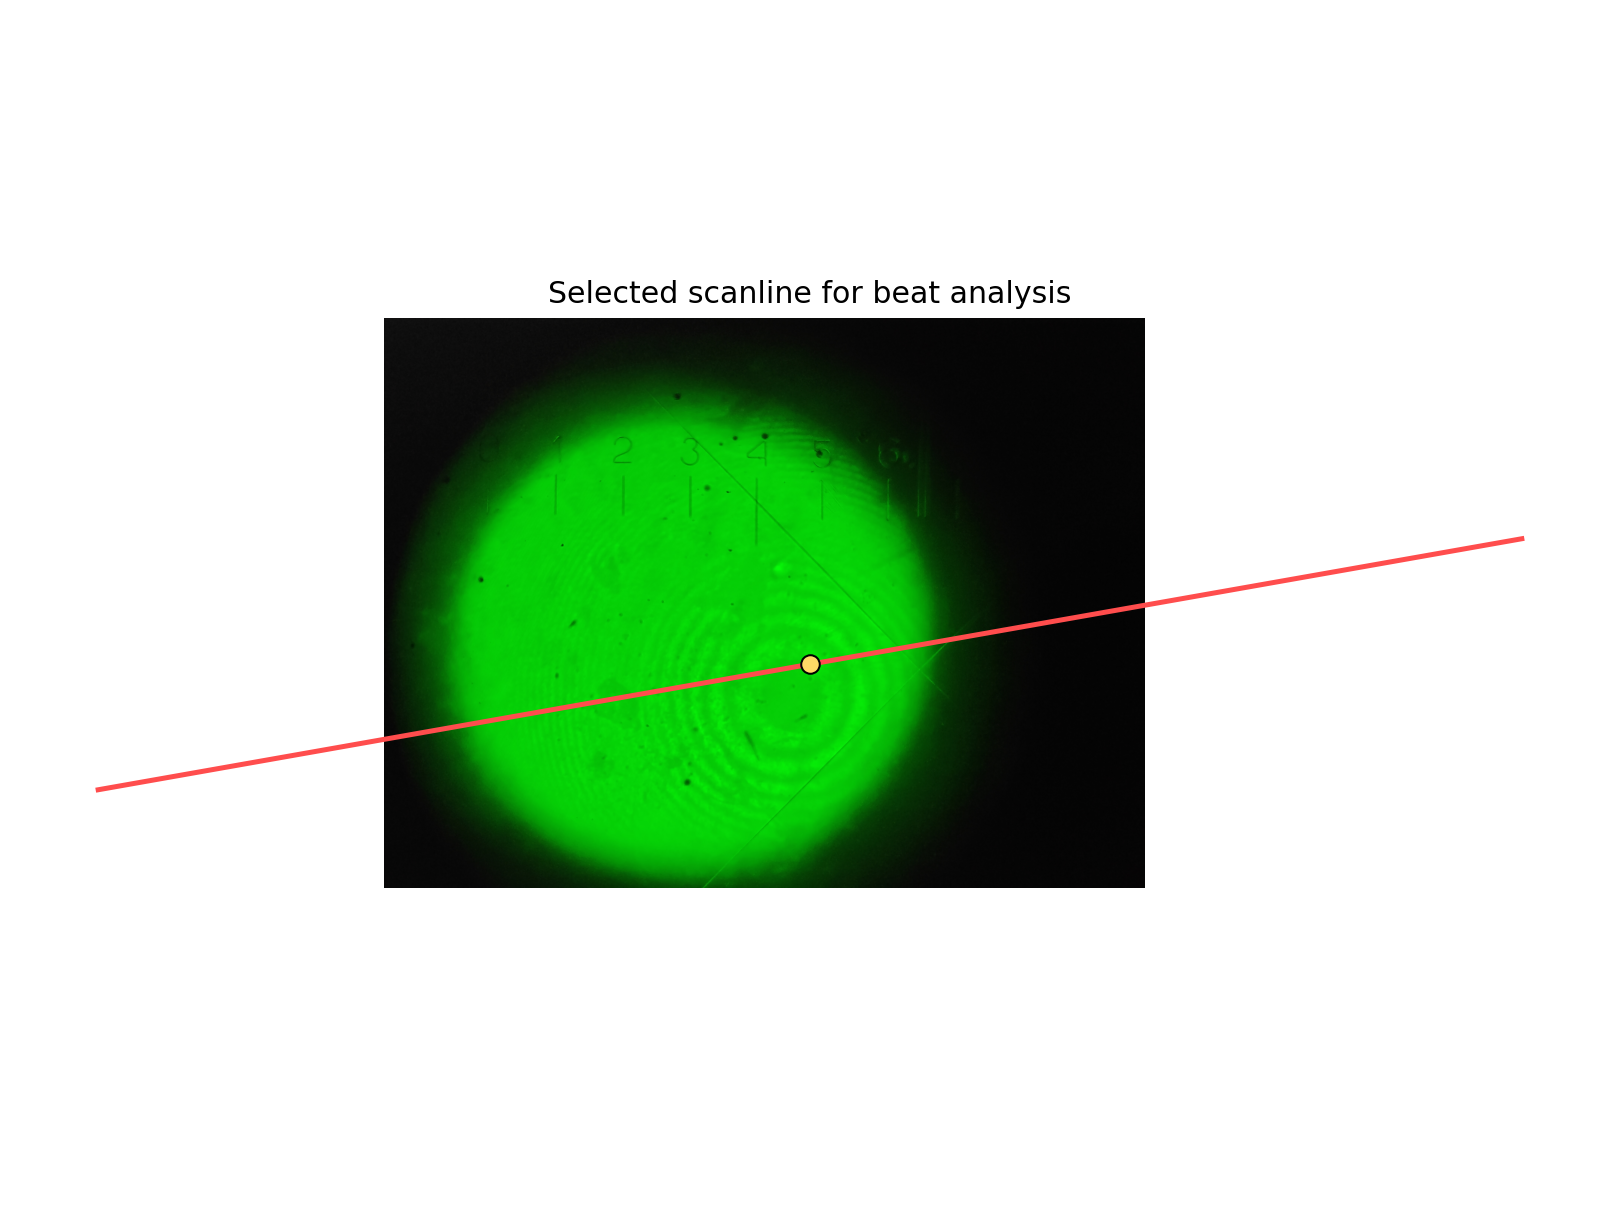
\includegraphics[width=0.78\textwidth]{beat_scanline.png}
\caption{Выбранный луч для анализа биений. Жёлтой точкой отмечен найденный центр пятна, красной линией --- луч, по которому строился профиль интенсивности.}
\end{figure}

\section*{Обсуждение результатов}

Основная неопределённость в определении радиуса кривизны связана с ручным восстановлением координат колец из таблицы измерений. Это видно по двум точкам, которые пришлось исключить из аппроксимации. После их исключения зависимость $r^2(n)$ становится почти линейной, а свободный член оказывается совместимым с нулём в пределах ошибки, что согласуется с теорией для тёмных колец.

Оценка по фотографии биений получилась устойчивой: на выбранном луче через центр пятна между соседними максимумами видности уверенно выделяются 17 тёмных колец. Полученное значение $\Delta \lambda = 32$ нм отличается от табличного $33$ нм менее чем на $3\%$, что для обработки по фотографии можно считать хорошим согласием.

\section*{Заключение}

В работе исследованы кольца Ньютона в отражённом свете и выполнена цифровая обработка фотографии картины биений.

По линейной зависимости $r_n^2(n)$ найден радиус кривизны линзы
\[
R = (1.6 \pm 0.1)\ \text{см}.
\]

По профилю интенсивности на фотографии биений получена оценка разности длин волн жёлтой и зелёной линий ртути
\[
\Delta \lambda = 32\ \text{нм},
\]
что хорошо согласуется с табличным значением $33$ нм.

\begin{thebibliography}{99}
\bibitem{labmanual}
Лабораторный практикум по общей физике: учеб. пособие. В 3 т. Т. 2. Оптика / А.\,В. Максимычев, Д.\,А. Александров, Н.\,С. Берюлёва и др.; под ред. А.\,В. Максимычева. М.: МФТИ, 2014. 446 с.
\end{thebibliography}

\end{document}
